% !TeX root = ../main.tex
% Add the above to each chapter to make compiling the PDF easier in some editors.

\chapter{Goal and Scope}\label{chapter:goal_req}
Developing a system to serve the purposes as introduced in the previous chapter is a complicated task that covers a wide area of knowledge and various domains. Therefore, it is essential to define the scope of the study, i.e., the goal it aims to achieve, and the scope which the key terms of it is supposed to cover.

\section{Goal}
The goal of this study is to find a method to create a stress-eating profile for a random individual based on his/her stress and eating data. More specifically, it tries to build a pipeline along which the following data can be collected via a conversational agent (which in this project is a chatbot) that interacts with its user on a daily basis:
\begin{itemize}
    \item Data on the individual’s stress level at the time of measurement, either detected by the conversational agent or reported by the individual through conversations
    \item Data on the individual’s level of stress during the days for a measurement period of more than two weeks
    \item Data on the individual’s food consumed when he/she was stressed at the time of measure, as self-reported by the individual to the conversational agent
    \item Data on the individual’s amount of food consumed during the days for a measurement period of more than two weeks
\end{itemize}
after which it builds a classification model for the individual based on the data collected that predicts whether the individual is likely to eat more or less under the influence of stress.

Furthermore, it is expected that the method can be applied to more users over a more extended period, and ultimately provide insights and input for other applications, such as a dietary adviser or a food recommendation system.

The following sections will define the scope of this project.

\section{Scope of Stress Detection} \label{scope_stress_detection}
Some of the most predominant research on stress detection (\cite{7_stress_detection, 8_stress_detection, 9_stress_detection}) all rely on sensor data. Sensors, especially those embedded in smart devices such as smartwatches and smart armbands, have the advantage of accessing health data, including heart rate, sleep, and physical exercises. Accessing such data is, on the one hand, non-intrusive, and on the other, hardly available by other forms of non-intrusive daily-used data-providers such as smartphone apps. Some smartphones are also equipped with such sensors, but their data quality is relatively poor, considering that users are not carrying the phone all the time. However, for this study, we chose not to utilize wearable smart devices because the data qualities provided by different smart devices vary. Meanwhile, this factor had to be controlled to obtain an accurate and unbiased prediction of stress across users.

Furthermore, no contextual information, such as GPS data and social activities being performed by the participants, was utilized. This decision was made because the chatbot platform (Rasa) (\cite{10_rasa}) and API (Telegram Bot API) (\cite{11_tg_bot_api}) chosen to be used do not support the gathering of such contextual data in the background. For example, to get the social activity a user is performing, the bot has to ask explicitly for where he/she is, whom he/she is with, and what exactly he/she is doing). More information on the choice of the framework can be found in \autoref{chapter:sys_design}. \bigskip

\noindent Instead, stress detection is done with a two-step process solely relying on simple conversations between the chatbot and the user. First, stress is sampled three times per day at fixed hours for every participant, i.e., the chatbot decides to ask about the user’s level of stress at these timestamps. Second, based on the answers collected from the users in the first two weeks, a weighted clustering algorithm is performed on the timestamps to determine the scheduled time of the coming day for stress detection. The number of clusters is determined by the stress states of the user in the past two days. If the user was stressed the day before, stress is going to be sampled three times the day after, hence three clusters. If the user was not feeling stressed the day before but was two days back, two clusters will be trained, leading to asking for stress twice in the coming day. Otherwise, only one cluster is going to be trained. \autoref{fig:adapt-stress} illustrates the way this adaptive stress-sampling works.

\begin{figure}[ht]
  \centering
  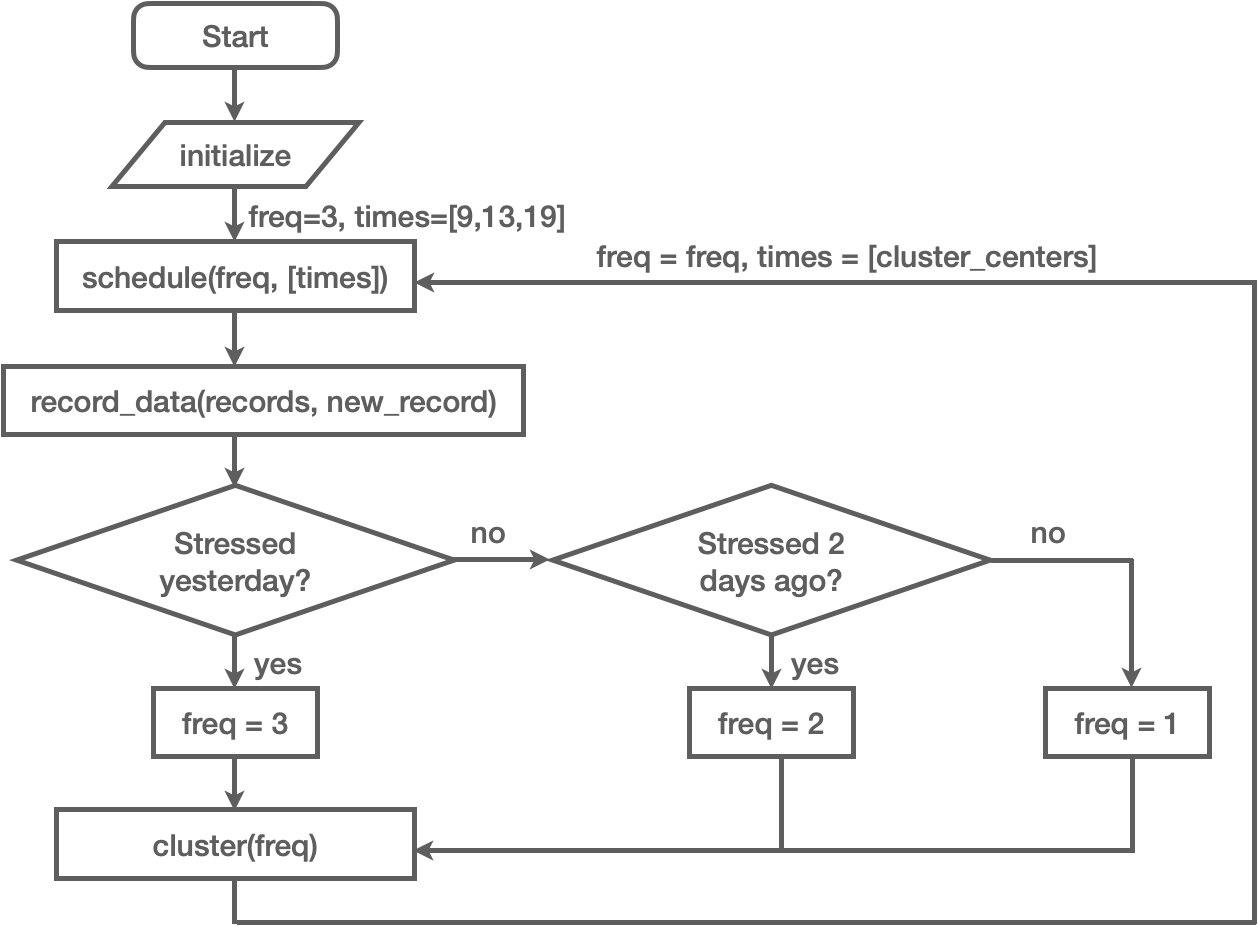
\includegraphics[width=0.7\textwidth]{fig-adapt-stress}
	\caption{The adaptive stress-sampling process}
	\label{fig:adapt-stress}
\end{figure}

\section{Scope of Stress Self-Reporting}

Users of the system have the option to actively report stress in the form of a conversation with the chatbot. The self-reporting uses natural language, and specifically in this project, English, as a natural language understanding (NLU) module in English is trained in this project. No other forms of interaction are involved.

\section{Definition of Eating Behaviors}

In this research, the so-called “eating behaviors” refer to patterns in food consumption. The scope of such patterns differs in two scenarios, under one of which is the data the system collects that is related to eating. This data is used as input to a supervised learning scheme that builds predictive models. Under the other scenario, i.e., when such models are put into use, “eating behaviors” refer to food consumption patterns of the participants and future users that the models try to predict.

In the first scenario, the chatbot collects both descriptive and categorical data. It asks the participants to describe the food consumed, in natural language, at the time when they are stressed, or at the end of the day. Besides, it invites the participants to reflect on the amount of food consumed during the day. In case the participants have been stressed during the day, it asks them to compare the food amount with that they are likely to eat when they are not stressed.

In the second scenario, the models try to predict only the categorical data related to food consumption, i.e., the amount of food likely to be consumed by a user given his/her stress level. Also, it tries to predict whether the user is expected to eat any comfort food, which is defined in the following section.

\section{Definition of Comfort Food}

The term “comfort food” is often used to describe food eaten by someone who is being stressed that offers comforting feelings to this person. However, it is often ambiguous, and its exact meaning differs in various contexts. \citeauthor{12_comfort_food_women, 14_comfort_food, 15_comfort_food_review} (\citeyear{12_comfort_food_women, 14_comfort_food, 15_comfort_food_review}) focused on different properties of comfort food, while agree on the fact that it often contains calorie-dense food. Among them, \citeauthor{14_comfort_food} (\citeyear{14_comfort_food}) offers a comprehensive categorization to comfort food into nostalgic foods, indulgence foods, convenience foods, and physical comfort foods. Comfort foods from all four categories are likely to be associated with stress relief, which is closely related to the topic of this research.

Since the chatbot was designed to be non-intrusive, it is unlikely to identify the social contexts the users are in and subsequently categorize the food they have eaten into one of the four categories \citeauthor{14_comfort_food} presented. However, as \citeauthor{14_comfort_food} also suggested, the definition of comfort food is highly personal. Therefore, this project invited the participants to define what comfort food is for themselves at an individual level. This method makes sense because, in the end, different models are built for each participant, and the definition of comfort food for one user is irrelevant to that for another. Technically, this was done by providing each user a survey towards the end of the chatbot trial (data collection phase), which contained all food items he or she had reported. The user, given the definition of comfort food, needed to label whether each food item is considered comfort food or not by himself or herself. Accordingly, each stress-eating entry was labeled with the binary value of being or not being comfort food, which became part of the training data.
